\documentclass{article}
\usepackage[utf8]{inputenc}
\usepackage{authblk}
\usepackage{setspace}
\usepackage[margin=1.25in]{geometry}
\usepackage{graphicx}
\usepackage{subfig}
\graphicspath{ {./figures/} }
\usepackage{subcaption}
\usepackage{amsmath}
\usepackage{hyperref}
\usepackage{titlesec}
\setcounter{secnumdepth}{4}
\usepackage{amssymb}
\usepackage[noend]{algpseudocode}
\usepackage{algorithm}
\usepackage{comment}
\usepackage{enumitem}
\usepackage{mathtools}
\usepackage{eucal} 
\usepackage{color}   %May be necessary if you want to color links

%%%%%% Bibliography %%%%%%
% Replace "sample" in the \addbibresource line below with the name of your .bib file.
\usepackage[style=ieee, 
citestyle=numeric-comp,
sorting=none]{biblatex}


\addbibresource{test.bib}
\numberwithin{equation}{section}


\title{Computational Mathematics for Learning and Data Analysis Project Report  A.Y. 2020/2021}


\author{Dawit Anelay}
\author{Marco Petix}
\author{Yohannis Telila}

%%%%%% Affiliations %%%%%%
\affil{Department of Computer science, University of Pisa, Pisa, Italy.}

%%%%%% Spacing %%%%%%
% Use paragraph spacing of 1.5 or 2 (for double spacing, use command \doublespacing)
\onehalfspacing

\titleformat{\paragraph}
{\normalfont\normalsize\bfseries}{\theparagraph}{1em}{}
\titlespacing*{\paragraph}
{0pt}{3.25ex plus 1ex minus .2ex}{1.5ex plus .2ex}
\setlength{\parindent}{0cm}

\begin{document}
\newtheorem{theorem}{Theorem}
\newtheorem{proposition}[theorem]{Proposition}
\maketitle

\tableofcontents

\begin{abstract}
(P) is the problem of estimating the matrix norm $\|A\|_2$, for a matrix $A \in R^{m\times n}$, using its definition as an (unconstrained) maximum problem.\\
(A1) is a conjugate gradient descent algorithm.\\
(A2) is a quasi-Newton method such as BFGS (one which does not require any approximations of the Hessian of the function).\\
(A3) is approximating the largest eigenvalue of $A^TA$ (or $AA^T$) using the Arnoldi process.
\end{abstract}

\section{The 2-Norm of a Matrix as a Maximization Problem}
We present the definition of the induced matrix 2-norm: 
\begin{equation}
    \|\boldsymbol{A}\|_2:=\sup_{\boldsymbol{x} \in \mathbb{R}^n_{\not = 0}}\frac{\|\boldsymbol{A} \boldsymbol{x}\|_2 }{\|\boldsymbol{x}\|_2}
\end{equation}
where the 2-norm is defined as: 
\begin{equation}
    \|\boldsymbol{x} \|_2 := \sqrt{\boldsymbol{x}^T \boldsymbol{x}} 
\end{equation}
and $\boldsymbol{A} \in \mathbb{R}^{m \times n}, \boldsymbol{x} \in \mathbb{R}^{n}_{\not =0}$.\\

By combining the previous definitions we can further detail the equation for $\| \boldsymbol{A}\|_2$ with:
\begin{equation}
    \|\boldsymbol{A}\|_2=\sup_{\boldsymbol{x} \in \mathbb{R}^n_{\not = 0}} \sqrt{\frac{(\boldsymbol{Ax})^T \boldsymbol{Ax}}{\boldsymbol{x}^T \boldsymbol{x}}}=\sup_{\boldsymbol{x} \in \mathbb{R}^n_{\not = 0}}\sqrt{\frac{\boldsymbol{x}^T \boldsymbol{A}^T \boldsymbol{A} \boldsymbol{x}}{\boldsymbol{x}^T \boldsymbol{x}}}
\end{equation}

Due to the monotone nature of the square root function, we can write :
\begin{equation}
    \|\boldsymbol{A}\|_2= \sup_{\boldsymbol{x} \in \mathbb{R}^n_{\not = 0}}  \frac{\boldsymbol{x}^T \boldsymbol{A}^T \boldsymbol{A} \boldsymbol{x}}{\boldsymbol{x}^T \boldsymbol{x}} 
\end{equation}

in order to express the estimation of the norm as the following unconstrained minimization problem:
\begin{equation}
    \|\boldsymbol{A}\|_2=\inf_{\boldsymbol{x} \in \mathbb{R}^n_{\not = 0}}  - f(\boldsymbol{x})
\end{equation}

Ultimately, we can define our objective function as:
\begin{equation}
    f(\boldsymbol{x})= - \frac{\boldsymbol{x}^T \boldsymbol{A}^T \boldsymbol{A} \boldsymbol{x}}{\boldsymbol{x}^T \boldsymbol{x}}
\end{equation}

\section{Properties of the Objective Function}
\subsection{Properties of $\boldsymbol{A}^T\boldsymbol{A}$}
Given a matrix $\boldsymbol{A}\in \mathbb{R}^{m\times n}$, the followings properties are valid for the matrix $\boldsymbol{A}^T\boldsymbol{A}$ (and $\boldsymbol{AA}^T$):
\begin{itemize}
\item The matrix is square: $\boldsymbol{A}^T\boldsymbol{A}\in \mathbb{R}^{n\times n}$
\item The matrix is symmetric: $(\boldsymbol{A}^T\boldsymbol{A})^T=\boldsymbol{A}^T(\boldsymbol{A}^T)^T=\boldsymbol{A}^T\boldsymbol{A}$
\item The matrix is positive semi-definite for any $\boldsymbol{x} \in \mathbb{R}^n$: $\boldsymbol{x}^T\boldsymbol{A}^T\boldsymbol{Ax}=(\boldsymbol{Ax})^T\boldsymbol{Ax}=\|\boldsymbol{Ax}\|_2$$ \geq$ 0

\end{itemize}
According to both the Spectral Theorem, which deals with the decomposition of the eigenvalues of symmetric matrices, and to the positive semi-definiteness of $\boldsymbol{A}^T\boldsymbol{A}$, we recognize said matrix as possessing only real and not negative eigenvalues.
\\
Ultimately, the properties of norms and matrices define the relationship between the spectral radius of $\boldsymbol{A}^T\boldsymbol{A}$, being the largest eigenvalues possessed by said matrix, and the 2-norm of matrix $\boldsymbol{A}$ as: 

\begin{equation}
    \|\boldsymbol{A}\|_2 = \sqrt{\rho(\boldsymbol{A}^T\boldsymbol{A})}
\end{equation} 

\subsection{Continuity, Differentiability and Gradient of the Function}
The domain of the objective function is $\mathbb{R}^n_{\not = 0}$ and, being it composed by simple and continuous functions, it results continuous within the same. 
\\

In order to compute the partial derivatives of the function at each step $i$, we express it as
\begin{equation}
    f(\boldsymbol{x})= - \frac{\boldsymbol{x^T M x}}{\boldsymbol{x^Tx}}= -  \frac{\sum_{i=1}^n \sum_{j=1}^n x_i m_{ij} x_j}{\sum_{i=1}^n x^2_i}
\end{equation}
where $m_{ij}$ are the elements of $\boldsymbol{M=A^TA}$.
\\
\begin{equation*}
\begin{aligned}
    \displaystyle \frac{\partial f}{\partial x_k}= - \frac{(\boldsymbol{x^T M x})'\boldsymbol{(x^Tx)}-(\boldsymbol{x^T M x})\boldsymbol{(x^Tx)'} }{(\boldsymbol{x^Tx})^2} \\ = -\frac{(\boldsymbol{2Mx})\boldsymbol{(x^Tx)} - (\boldsymbol{x^T M x})2x }{(\boldsymbol{x^Tx})^2} \hspace{1.1cm} \\ =\frac{2x(\boldsymbol{x^T M x})}{(\boldsymbol{x^Tx})^2}-\frac{ \boldsymbol{2Mx}}{ \boldsymbol{x^Tx}}\hspace{2.6cm}  
\end{aligned}
\end{equation*}

We can write our partial derivative result as:

\begin{equation}
    \displaystyle \frac{\partial f}{\partial x_k}=\frac{2x_k (\sum_{i=1}^n \sum_{j=1}^n x_i m_{ij}x_j)}{(\sum_{i=1}^n x_i^2)^2} - \frac{ \sum_{j=1}^n  m_{kj}x_j}{ \sum_{i=1}^n x_i^2} = \frac{2x_k(\boldsymbol{x^T Mx})}{(\boldsymbol{x^Tx})^2} - \frac{ \boldsymbol{2Mx}}{\boldsymbol{x^Tx}}  
\end{equation}

The derivative of our objective function exist, are continuous and differentiable in all points expect 0. The objective function is therefore differentiable in $\mathbb{R}^n \setminus \{0\}$.

We can write the gradient of the function as

\begin{equation}
    \nabla f(\boldsymbol{x})= \frac{2 \boldsymbol{x}( \boldsymbol{x^T M x})}{(\boldsymbol{x^Tx})^2} - \frac{ \boldsymbol{2Mx}}{ \boldsymbol{x^Tx}}
\end{equation}

\subsection{Complexity of the Function and its Gradient}

Computing $\boldsymbol{M}$ would require $O(m^2n)$ operations but its symmetric nature simplifies this process by halving the amount of elements actually needed, also, such computation is only required once. \\

Computing $\boldsymbol{x^TM}$ instead requires $O(n^2)$ operations and the same is valid for the computation of $(\boldsymbol{x^TM})\boldsymbol{x}$ too. Finally, computing $\boldsymbol{x^T}\boldsymbol{x}$ and the division take $O(n)$ and $1$ operations. \\The total complexity of the function is therefore
\begin{equation}
    C(f(\boldsymbol{x}))=2 O(n^2)+O(n)+1=O(n^2)
\end{equation}

Computing the first term of the gradient takes $O(n^2) + O(n^2) + 1$ operations, computing the second term instead takes $3 O(n^2) + 2 O(n^2) + 1$. Ultimately, the total complexity of the gradient of the function is
\begin{equation}
    C(\nabla f(\boldsymbol{x}))=7 O(n^2)+3 = O(n^2).
\end{equation}

It's still possible to reduce such complexity by rewriting the gradient as

\begin{equation}
    \nabla f(\boldsymbol{x})= \frac{ \boldsymbol{2Mx}}{ \boldsymbol{x^Tx}} - \frac{2 \boldsymbol{x}(f(\boldsymbol{x}))}{\boldsymbol{x^Tx}}=\frac{ \boldsymbol{Mx} - 2 \boldsymbol{x}(f(\boldsymbol{x}))}{ \boldsymbol{x^Tx}}.
\end{equation}

This enables the use of the values already computed for $f(\boldsymbol{x})$, $\boldsymbol{Mx}$ and $\boldsymbol{x^Tx}$ and limits the task of obtaining the gradient to the single computation of $\boldsymbol{x}f(\boldsymbol{x})$.

The complexity of computing the gradient, after applying the aforementioned transformations, is
\begin{equation}
    C(\nabla f(\boldsymbol{x}))=O(n).
\end{equation}

\subsection{Stationary Points}

Another important property we want to know about our function is whether it has a stationary point because we want our algorithm to converge to these points. Lets say our stationary point $\boldsymbol{\hat{x} \neq 0}$, we are interested to find where $\nabla f(\hat{x}) = 0$


\begin{equation}
    \nabla f(\hat{\hat{\boldsymbol{x}}})= \frac{ \boldsymbol{2M\hat{\boldsymbol{x}}}}{ \boldsymbol{\hat{\boldsymbol{x}}^T\hat{\boldsymbol{x}}}} - \frac{2 \hat{\boldsymbol{x}}( \boldsymbol{\hat{\boldsymbol{x}}^T M \hat{\boldsymbol{x}}})}{(\boldsymbol{\hat{\boldsymbol{x}}^T\hat{\boldsymbol{x}}})^2}=\frac{\boldsymbol{2M\hat{\boldsymbol{x}}}(\boldsymbol{\hat{\boldsymbol{x}}^T\hat{\boldsymbol{x}}}) -  2 \hat{\boldsymbol{x}}( \boldsymbol{\hat{\boldsymbol{x}}^T M \hat{\boldsymbol{x}}})}{(\boldsymbol{\hat{\boldsymbol{x}}^T\hat{\boldsymbol{x}}})^2}=0
\end{equation}
\begin{equation}
    \boldsymbol{2M\hat{\boldsymbol{x}}}(\boldsymbol{\hat{\boldsymbol{x}}^T\hat{\boldsymbol{x}}}) -  2 \hat{\boldsymbol{x}}( \boldsymbol{\hat{\boldsymbol{x}}^T M \hat{\boldsymbol{x}}})=0
\end{equation}
\begin{equation}
    \boldsymbol{2M\hat{\boldsymbol{x}}}(\boldsymbol{\hat{\boldsymbol{x}}^T\hat{\boldsymbol{x}}}) = 2 \boldsymbol{\hat{\boldsymbol{x}}}( \boldsymbol{\hat{\boldsymbol{x}}^T M \hat{\boldsymbol{x}}})
\end{equation}

We can remove 2 from both sides.

\begin{equation}
    \boldsymbol{M\hat{\boldsymbol{x}}}(\boldsymbol{\hat{\boldsymbol{x}}^T\hat{\boldsymbol{x}}}) =  \boldsymbol{\hat{\boldsymbol{x}}}( \boldsymbol{\hat{\boldsymbol{x}}^T M \hat{\boldsymbol{x}}})
\end{equation}

\begin{equation}
    \frac{ \boldsymbol{\hat{\boldsymbol{x}}}( \boldsymbol{\hat{\boldsymbol{x}}^T M \hat{\boldsymbol{x}}})}{(\boldsymbol{\hat{\boldsymbol{x}}^T\hat{\boldsymbol{x}}})} = \boldsymbol{M\hat{\boldsymbol{x}}}
\end{equation}
\begin{equation}
     f(\boldsymbol{\hat{\boldsymbol{x}}})\boldsymbol{\hat{\boldsymbol{x}}} = \boldsymbol{M\hat{\boldsymbol{x}}}
\end{equation}


We can say that $\hat{x}$ is stationary point for our function if and only if $\hat{x}$ is eigen vector for $\boldsymbol{M}$ and its eigenvalue is $f(\boldsymbol{\hat{\boldsymbol{x}}})$.

\subsection{Bounds on the Function and descent direction}

Another important property of our function is that the function is bounded.   
\begin{equation*}
    \exists D \in \mathbb{R^+} \quad s.t \quad |f(x)| \leq D
\end{equation*}
\begin{equation*}
   \left \| -f(x) \right \| = \left \| \frac{x^TMx}{x^Tx} \right \|
  \end{equation*}
 We can expand the norm using Cauchy-Schwarz inequality as follow
 \begin{equation}
  \left \| \frac{x^TMx}{x^Tx} \right \| \leq \frac{\left \| x^T \right \|\left \| M \right \|\left \| x \right \|}{\left \| x \right \|^2} \leq \left \| M \right \| \leq D
 \end{equation}

Next we discuss the closed formula to  compute the step-size $\alpha ^i$ at given point \textbf{$x^i$} at the $i^{th}$ iteration along the direction $d^i$. 

 \begin{equation*}
   \varphi(\alpha ^i) = \arg \min {f(x+\alpha ^i d ^i)}
\end{equation*}

So we are looking for the minimum of this function $\varphi(\alpha^i)$ and the minimum of the function can be found by solving $\varphi'(\alpha^i)=0$ equation.  We have the equation for $f(x)$ and $\triangledown f(x)$ from equation 8 and 10.

 \begin{equation*}
 \begin{aligned}
   &\varphi(\alpha) = f(x(\alpha)),\hspace{0.15cm} where \hspace{0.15cm} x(\alpha) = x+\alpha d  \\
   &f(x(\alpha)) = \frac{-(x+\alpha d)^TM(x+\alpha d)}{(x+\alpha d)^T(x+\alpha d)} \\
   &\varphi(\alpha) =  -(\frac{x^TMx + \alpha (d^TMx + x^TMd) + \alpha^2(d^TMd)}{x(\alpha)^Tx(\alpha)}) \\
   \end{aligned}
\end{equation*} 

But $x^TMd \in 	\mathbb{R} $ and $M$ is symmetric, means that $x^TMd = (x^TMd)^T = d^TM^Tx = d^TMx$. Hence the above equation can be written as below.

 \begin{equation*}
 \begin{aligned}   
   \varphi(\alpha) = -(\frac{x^TMx + 2\alpha d^TMx + \alpha ^2 d^TMd}{x(\alpha)^Tx(\alpha)})  
   \end{aligned}
\end{equation*} 

 \begin{equation*}
 \begin{aligned}   
  \varphi ' (\alpha) = -[\frac{(2d^TMx + 2\alpha d^TMd)(x(\alpha)^Tx(\alpha)) - ((x^TMx + 2\alpha d^TMx + \alpha ^ 2 d^TMd)(2(x+\alpha d)^Td))}{(x(\alpha)^Tx(\alpha))^2}] \\
   \end{aligned}
\end{equation*} 
\begin{equation*}
\hspace{-3.60cm}  = -\big[ 2 \alpha ^3 ((d^TMd)d^Td) + 2\alpha ^2((d^TMx)d^Td + 2(d^TMd)d^Tx) + 
\end{equation*} 
\begin{equation*}
 \hspace{-3.40cm} 2\alpha((d^TMd)x^Tx) + 2((d^TMx)d^Tx) + 2((d^TMx)x^Tx) \big] +
\end{equation*}
\begin{equation*}
 \hspace{-3.0cm}   \big[ 2\alpha ^3((d^TMd)d^Td) + 2\alpha^2((d^TMx)d^Td + 2(d^TMx)d^Td) + 
\end{equation*}
\begin{equation*}
\hspace{-3.25cm} \frac{2\alpha(2(d^TMx)(x^Td)) + (x^TMx)d^Td) + 2((x^TMx)x^Td)\big]}{(x(\alpha)^Tx(\alpha))^2}
\end{equation*}
By simplifying the above equation we would have
\begin{equation*}
\varphi '(\alpha) = \frac{2\alpha ^2 ((d^TMx)d^Td -(d^TMd)d^Tx) + 2\alpha((x^TMx)d^Td) - (d^TMx)x^Tx) + 2(x^TMx)x^Td - (d^TMx)x^Tx}{((x+\alpha d)^T(x+\alpha d))^2}
\end{equation*} 
We can write our equation in a short form like this
\begin{equation*}
\varphi '(\alpha) = 2 .\frac{\alpha ^2 a + \alpha b + c }{R(\alpha)}
\end{equation*}

Where,
\begin{equation}
\hspace{-10.90cm} a = (d^TMx)d^Td 
\end{equation}
\begin{equation*}
\hspace{-8.30cm} b = ((x^TMx)d^Td - (d^TMd)(x^Tx)) 
\end{equation*}
\begin{equation*}
\hspace{-8.5cm} c = (x^TMx)x^Td - (d^TMx)x^Tx
\end{equation*}
\begin{equation*}
 \hspace{-10.20cm} R(\alpha) = (x(\alpha)^Tx(\alpha))^2
\end{equation*}

To discuss the complexity of computing this, In general to calculate the parameters a,b and c it takes $\mathcal{O}(n^2)$ because obtaining the value for $x^TMx$ and $d^TMd$ requires $\mathcal{O}(n^2)$ complexity.

\begin{equation}
 \mathcal{C}(\varphi '(\alpha)) = \mathcal{O}(n^2)
\end{equation}

\subsection{Non Convexity of the Function}

 Our function cannot be convex because the only function that is bounded and convex is a constant function; Our function is bounded but not constant for this reason we can say that our function is not convex. \\
 If we make an assumption that \begin{math} f(x) \end{math} is convex, \begin{math} \triangledown {f(x)} \end{math} exists almost everywhere and the following inequality holds.
 \begin{equation*}
    f(y) \geq f(x) + \langle \triangledown f(x),y-x \rangle \quad \forall x,y \in R^n
\end{equation*}
      
If we take two different eigenvalues $\Tilde{x}_i$ \,\, and \,\,\, $\Tilde{x}_j$ with $f(\Tilde{x}_i) \,\,$ and $\,\,f(\Tilde{x}_j)$ eigenvectors and if we assume $\Tilde{x}_i >  \Tilde{x}_j$, then $f(\Tilde{x}_i) \,\, > \,\,f(\Tilde{x}_j)$. But from the convex inequality assumption stated above, we would get $f(\Tilde{x}_i) \,\, \leq \,\,f(\Tilde{x}_j)$, which contradicts the convexity hypothesis.


\section{Conjugate gradient method}

Conjugate gradient method is one of the optimization techniques. In this section we will be showing how we can use this method to optimize our function. The algorithm of the conjugate gradient method is defined as below.

\begin{algorithm}
\caption{Pseudo-code for Conjugate Gradient Method}\label{alg:cgm}
\begin{algorithmic}[1]
\Procedure{CGM}{$x_0,\epsilon$}\Comment{The cgm}
\State \begin{math} d_0\gets -\triangledown f(x_0) \end{math}
\While{$\|\boldsymbol{\triangledown f(x_k)}\| > \epsilon $}
\State$\beta _k = \frac{\triangledown f(x_k)^{T}\triangledown f(x_k)}{\triangledown f(x_{k-1})^{T}\triangledown f(x_{k-1})} $
\State $ d_k = - \triangledown f(x_k) + \beta _k d_{k-1} $
\State $ \varphi(\alpha) = f(x_k + \alpha d_k)$
\State $ \alpha _k = \underset{\alpha}{min} \varphi ^{'} (\alpha) $
\State $ x_{k+1} =  x_k + \alpha _k d_k$
\EndWhile\label{cgmendwhile}
\State \textbf{return} $x_{k+1}$
\EndProcedure
\end{algorithmic}
\end{algorithm}

We used Fletcher-Reeves method to calculate the value for $\boldsymbol{\beta _k}$.

\subsection{Exact search along the direction $d_k$}
$\boldsymbol{d_k}$ is our descent direction and the exact search along this direction is given as, $\varphi^{'}(\alpha) = 0 $.

 \begin{equation*}
   \varphi^{'}(\alpha) = \triangledown f(\boldsymbol{x_{k+1}})^{T}\boldsymbol{d_k}
\end{equation*}

We can also prove that the gradient and the descent direction are of the opposite direction.

\begin{equation*}
\begin{aligned}
    & \triangledown f(x_k)^{T}{d_k} \leq 0 \\
    & \triangledown f(x_k)^{T} (- \triangledown f(x_k) + \beta _k d_{k-1}) \leq 0 \\
    & - \triangledown f(x_k)^T\triangledown f(x_k) + \beta _k \triangledown f(x_k)^{T}d_{k-1} \leq 0 \\
    & - \left \| \triangledown f(x_k) \right \|_2^2 + \beta _k \triangledown f(x_k)^{T}d_{k-1} \leq 0 
\end{aligned}
\end{equation*}

\begin{math} \triangledown f(x_k) \end{math} and \begin{math} d_{k-1} \end{math} are orthogonal. So, this value will always be less than 0. \\

As we have proved in the section 2.5 we can obtain the value $\alpha$ along the descent direction $d$ that minimizes the function $\varphi (\alpha) = f(x+\alpha x)$ is given by 

\begin{equation*}
 \hspace{-7.90cm} \frac{\alpha^2 a + \alpha b + c}{R(\alpha)} = \varphi '(\alpha) = 0
\end{equation*}

Where,
\begin{equation}
\hspace{-10.90cm} a = (d^TMx)d^Td 
\end{equation}
\begin{equation*}
\hspace{-8.30cm} b = (x^TMx)d^Td - (d^TMd)(x^Tx) 
\end{equation*}
\begin{equation*}
\hspace{-8.5cm} c = (x^TMx)x^Td - (d^TMx)x^Tx
\end{equation*}
\begin{equation*}
 \hspace{-10.20cm} R(\alpha) = (x(\alpha)^Tx(\alpha))^2
\end{equation*}


One important thing to notice is that $R(\alpha) \neq 0$

\begin{equation*}
\begin{aligned}
    R(\alpha) \neq 0 \\
 ((x+\alpha d)^T(x+\alpha d)) \neq 0 \\
 \|x+\alpha d \|^2_2 \neq 0 \\
 x^Tx + \alpha ^2d^Td + 2\alpha <x,d> \neq 0
\end{aligned}
\end{equation*}
Note : In CGD instead of $d$ we use $p$. So, $R(\alpha) = \|x_k + \alpha_k p_k\|_2^2$  \\
For $R(\alpha)$ to be 0 all the three equation $x^Tx$ , $\alpha ^2d^Td$ and $2\alpha <x,d>$ has to be 0 or if $x^Tx$ , $\alpha ^2d^Td$ are positive, $2\alpha <x,d>$ should not be negative. But, $x^Tx = \|x_k\|_2^2$ and $\|p_k\|_2^2$ are always greater or equal to 0. So, If we can show that $2\alpha <x,d>$ is always greater than 0, $R(\alpha)$ is always different from 0. Using Cauchy–Schwarz inequality we can show that
 \begin{equation*}
 |<x_k, p_k>| < \|x_k\|_2^2\|p_k\|_2^2
\end{equation*}

Since the sign is less than, that mean the cosine angle between the two is not 1(or -1) hence, not linearly dependant.
\\
So now we showed that $R(\alpha) \neq 0 $, we now want to find a solution for $\phi ' (\alpha) = 0$ \\
 \begin{equation}
 a\alpha^2 + b\alpha + c = 0
\end{equation}
\subsection{Convergence of the Algorithm}

Lets first consider this assumption:

The level set $\mathcal{L}$:=\{$x$\in $\mathbb{R}^n:$ $f(x)$ $\leq$ $f(x_0)$\} is bounded. This guarantees us a bound for the $\|x_k\|$. So, we want to  prove that the iterates remain bounded away from 0 by some constant positive number. Given $D = \mathbb{R}^n \char`\\  B(0,\varepsilon)$ and $x_k \in D$ , we want to show $\|x_k\|_2 \geq \epsilon > 0, \forall k \geq 0$. \\

We started with the assumption that $\|x_o\|_2^2 \geq \epsilon > 0$, and now lets compute for $\|x_1\|_2$.
\begin{equation*}
\|x_1\|_2^2 =  \|x_0 + \alpha _0 p_0\|_2^2 > 0 \\
   = \|x_0\|_2^2 +2\alpha_0 <x_0,p_0>+ \alpha_0^2\|p_0\|_2^2   > 0 \\
\end{equation*}

But this term  $2\alpha_0 <x_0,p_0>$ is 0 since $p_0 = -\triangledown f(x_0)$  and $\|x_0\|_2^2 > 0$. So its true that $\|x_1\|_2 > 0$

We can do the same for $\|x_2\|_2$. If we generalize for $\|x_k\|_2^2$, we would get.

\begin{equation*}
\|x_k\|_2 =  \|x_{k-1} + \alpha _{k-1} p_{k-1}\|_2^2 > 0 \\
   = \|x_{k-1}\|_2^2 +2\alpha_{k-1} <x_{k-1},p_{k-1}>+ \alpha_{k-1}^2\|p_{k-1}\|_2^2   > 0 \\
\end{equation*}


\begin{equation}
<x_k,p_k> = \sum_{i=0}^{k-1} \big(\prod_{j=k+1-i}^{k+1}\beta_j\big) \hat{\alpha _i} \|p_i\|_2^2 > 0 , \forall i 
\end{equation}
Hence, $\forall k , \|x_k\|_2^2 > 0 \Rightarrow \exists \epsilon $ s.t $\|x_k\|_2^2 \geq \epsilon$. That means $\|x_k\|_2^2$ bounded from below. Moreover, using triangle inequality, hölder's inequality and Cauchy–Schwarz inequality it is possible to show that the gradient is bounded by some constant.

\begin{equation}
 \|\triangledown f(x)\| \leq 4\|M\|^2 , \|x\|=1 
\end{equation}

\begin{proposition}
If a function $f$ has bounded derivative, then $f$ is lipschitz continuous.
\end{proposition}

Assuming we have $\alpha$ that satisfies Wolfe's condition and using the proof provided by Zoutendijk’s theorem with Fletcher–Reeves and Polak–Ribiere methods we can guarantee that our algorithm will converge to a stationary point given that our function is bounded from below in $R^n$(2.15), continuously differentiable (2.4) and lipschitz continuous(Proposition 1). The complete proof is provided at  \cite[pg.~127-131]{1}.


\subsection{Complexity of the Algorithm}
For CGD we have computation for $\beta _k$ and $P_k$ which we can obtain both with $\mathcal{O}(n)$ complexity. We have proved the complexity for $f(x), \triangledown f(x)$ and $ \phi ' (\alpha)$ in the previous sections. So we can say that the complexity of one iteration of the conjugate gradient method is $\mathcal{O}(n^2)$
 \begin{equation}
 C(CGD) = \mathcal{O}(n^2)
\end{equation}


\subsection{Performance of Algorithm}
In this section we will provide performance analysis of our algorithm implementation. For this purpose we have generated the following matrices with different properties. $x_0$ ($b_0$ in case of arnoldi) is the initial guess for the specified matrix. We ran all our experiments on Apple Macbook Air(Early 2014) 1.4 GHz Dual-Core Intel Core i5 with 4 GB 1600 MHz DDR3 memory.

\begin{itemize}
    \item \textbf{[M1]} is ill-conditioned matrix  $A_{1000\times1000}$, where a $\in$ \lbrack-2,3\rbrack and cond. no = 2e15, $x_0 \in \mathbb{R}^{1000}$.
    \item \textbf{[M2]} $A_{10000\times100}$, where a $\in$ \lbrack-50,50\rbrack ,  $x_0 \in \mathbb{R}^{100}$ vector.
    \item \textbf{[M3]} $A_{100\times1000}$, where a $\in$ \lbrack-50,50\rbrack ,  $x_0 \in \mathbb{R}^{1000}$ vector.
    \item \textbf{[M4]} $A_{100\times100}$, where a $\in$ \lbrack-50,50\rbrack , $x_0 \in \mathbb{R}^{100}$ vector.
    \item \textbf{[M5]} is sparse matrix  $A_{1000\times100}$ and density = 0.3, $x_0 \in \mathbb{R}^{100}$.
\end{itemize}

 For this experiment we randomly generated our initial guess with a range of \lbrack-50,50\rbrack . We set the value for maximum iteration to be 1000 and 1e-5 for epsilon. For minimum step size $\alpha$ we chose 1e-8. Residual is defined as the norm of the gradient and relative error is defined as the ratio between absolute error and accepted norm. They are defined as follow.
 
 \begin{equation}
    \begin{multlined}
     ~~~Residual = \|\triangledown f(x^i)\|\\
     Relative Error = (f(x^i) - f^*) / |f^*|
    \end{multlined}
\end{equation}

 
 Figure \ref{fig:err_m1},\ref{fig:err_m2},\ref{fig:err_m3},\ref{fig:err_m4} and \ref{fig:err_m5} shows relative error and residual generated by the algorithm with different methods on our test matrices.

\begin{figure}[H]
    \centering
    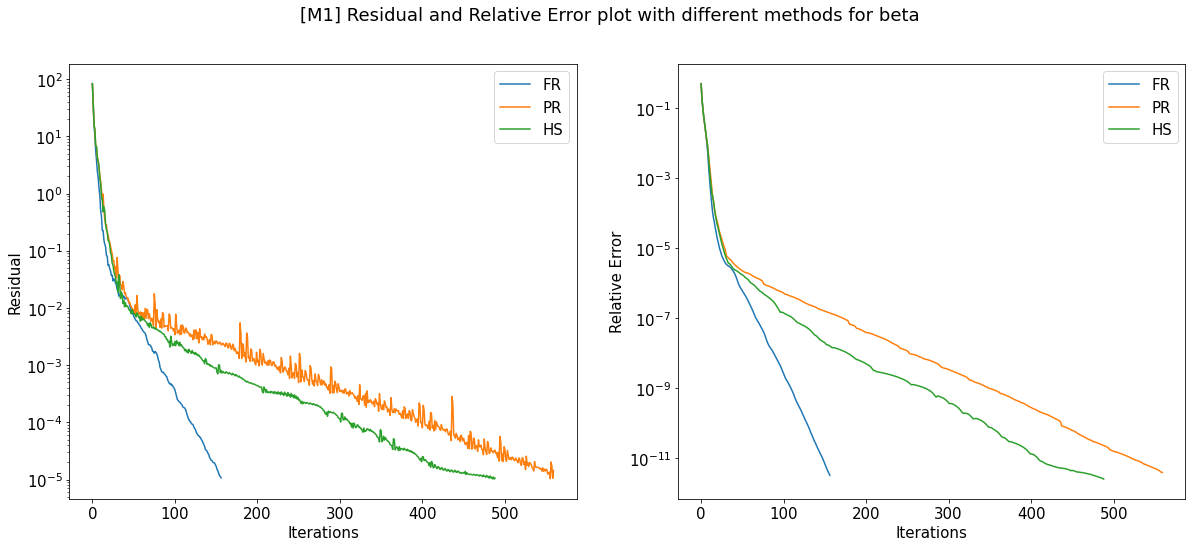
\includegraphics[scale=0.28]{cgd/M1.png}
    \caption{Relative error and residual plot for M1 matrix}
    \label{fig:err_m1}
\end{figure}

\begin{figure}[H]
    \centering
    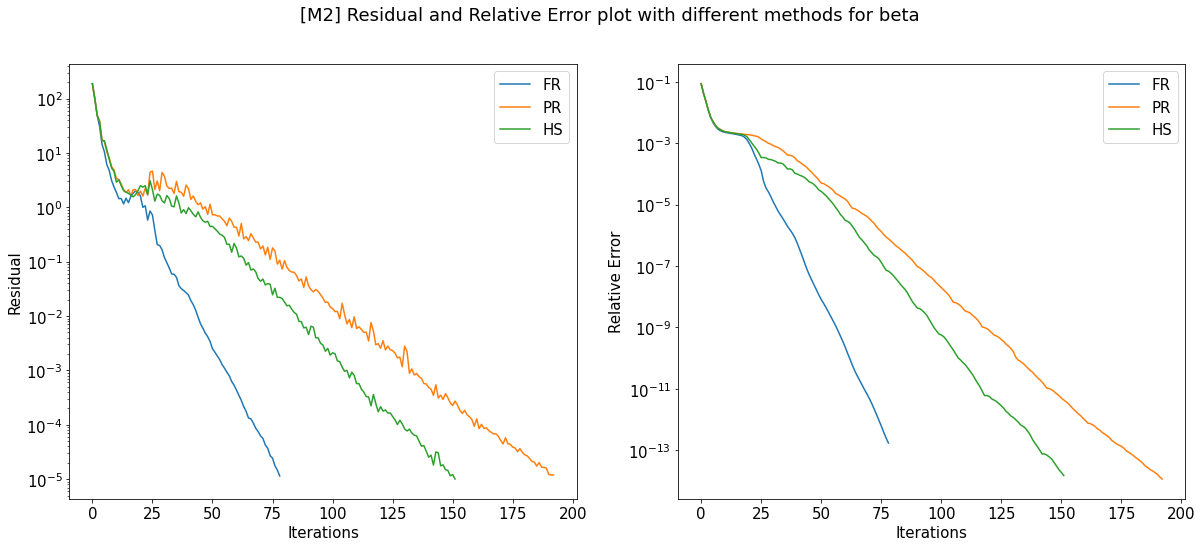
\includegraphics[scale=0.25]{cgd/M2.png}
    \caption{Relative error and residual plot for M2 matrix}
    \label{fig:err_m2}
\end{figure}

\begin{figure}[H]
    \centering
    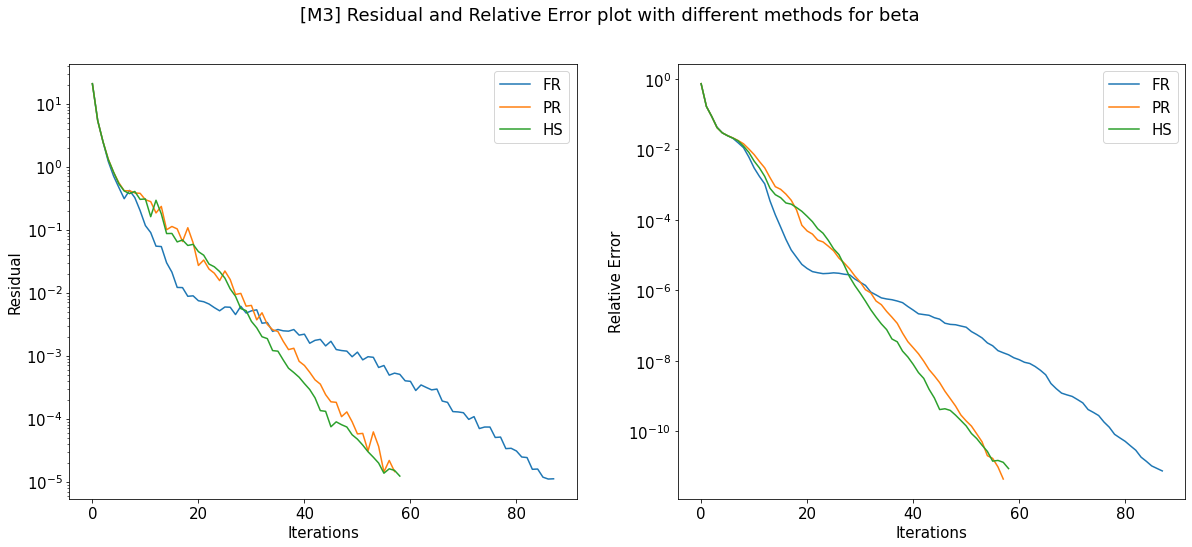
\includegraphics[scale=0.25]{cgd/M3.png}
    \caption{Relative error and residual plot for M3 matrix}
    \label{fig:err_m3}
\end{figure}

\begin{figure}[H]
    \centering
    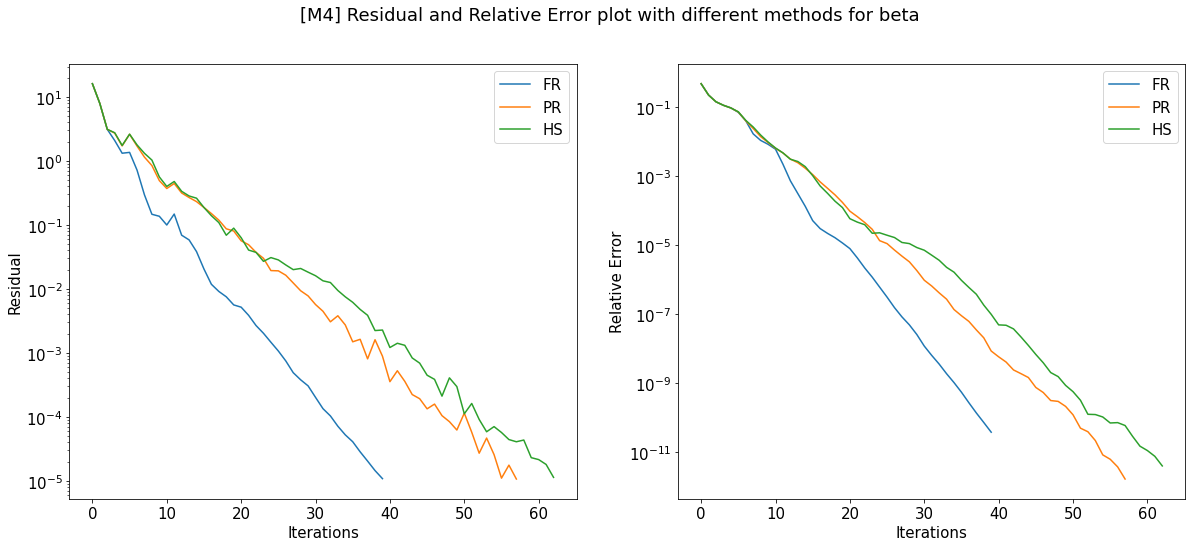
\includegraphics[scale=0.24]{cgd/M4.png}
    \caption{Relative error and residual plot for M4 matrix"}
    \label{fig:err_m4}
\end{figure}

\begin{figure}[H]
    \centering
    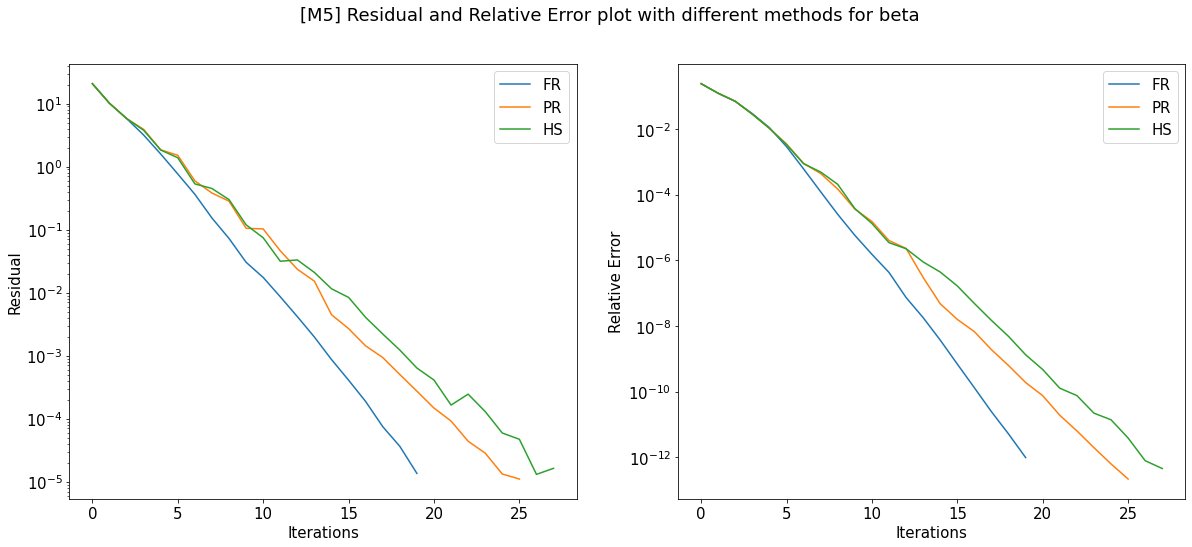
\includegraphics[scale=0.25]{cgd/M5.png}
    \caption{Relative error and residual plot for M5 matrix}
    \label{fig:err_m5}
\end{figure}



Looking at all Fig. \ref{fig:err_m1}, Fig. \ref{fig:err_m2} and Fig. \ref{fig:err_m3} we can understand that the algorithm converges faster and doesn't show significant change in both error and residual. So, it would be possible to do an early stopping even before $1e\-{-5}$ without affecting the final result significantly. We can also observe that our algorithm converges slower on ill conditioned matrices.
\subsubsection{Algorithm time performance}
We evaluated the running time performance of our algorithm and compared the accuracy of the result with numpy linear algebra implementations of a method norm \footnote{https://numpy.org/doc/stable/reference/generated/numpy.linalg.norm.html}. The following table summarises the running time of our implementation compared to the numpy tool. The error column represents the absolute difference between the solution provided by our algorithm and the numpy norm library.

\begin{table}[hbt!]
    \centering
    \begin{tabular}{||c c c c c||}
 \hline
 Matrix & CGD(Time) & np.linalg.norm(Time) & Relative Error & Iterations \\ [0.8ex] 
 \hline\hline
 M1 & 834 ms ± 146 ms & 537 ms ± 23.7 ms & 2.87e-12 & 157 \\
 
 \hline
 M2 & 23.9 ms ± 1.53 ms & 79.3 ms ± 2.24 ms & 1.14e-13 & 79\\
 \hline
 M3 & 336 ms ± 22.4 ms & 12.7 ms ± 2.23 ms & 5.24e-12 & 88 \\
 \hline
 M4 & 14.1 ms ± 491 µs & 1.83 ms ± 401 µs & 2.01e-11 & 40 \\
 \hline
 M5 & 7.57 ms ± 1.46 ms & 5.74 ms ± 691µs & 2.57e-13 & 20 \\
 \hline
\end{tabular}
    \caption{Time performance, epsilon = 1e-5 and beta = "FR"}
    \label{tab:fr_table}
\end{table}


\begin{table}[hbt!]
    \centering
    \begin{tabular}{||c c c c c||}
 \hline
 Matrix & CGD(Time) & np.linalg.norm(Time) & Relative Error & Iterations \\ [0.8ex] 
 \hline\hline
 M1 & 2.41 s ± 472ms & 585 ms ± 42.3 ms & 3.78e-12 & 560\\ 
 \hline
 M2 & 86.2 ms ± 35.1 ms & 81.8 ms ± 1.98 ms & 0.0069 & 193\\
 \hline
 M3 & 226 ms ± 14 ms & 11.5 ms ± 2.17ms  & 2.58e-12 & 89  \\
 \hline
 M4 & 17.2 ms ± 1.2 ms & 1.41 ms ± 60.9µs & 1.17e-12 & 58 \\
 \hline
  M5 & 7.75 ms ± 295 µs & 8.78 ms ± 2.31 ms & 6.33e-14 & 26 \\
 \hline
\end{tabular}
    \caption{Time performance, epsilon = 1e-5 and beta = "PR"}
    \label{tab:pr_table}
\end{table}

\begin{table}[hbt!]
    \centering
    \begin{tabular}{||c c c c c||}
 \hline
 Matrix & CGD(Time) & np.linalg.norm(Time) & Relative Error & Iterations \\ [0.8ex] 
 \hline\hline
 M1 & 3.11 s ± 311ms & 585 ms ± 42.3 ms & 2.44e-12 & 490\\ 
 \hline
 M2 & 54.9 ms ± 13.8 ms & 81.8 ms ± 1.98 ms & 1.23e-14 & 153\\
 \hline
 M3 & 285 ms ± 25.4 ms & 11.5 ms ± 2.17ms  & 6.048e-12 & 60  \\
 \hline
 M4 & 26.1 ms ± 1.63 ms & 1.41 ms ± 60.9µs & 2.20e-12 & 64 \\
 \hline
  M5 & 10.1 ms ± 295 µs & 8.78 ms ± 2.31 ms & 1.2e-13 & 29 \\
 \hline
\end{tabular}
    \caption{Time performance, epsilon = 1e-5 and beta = "HS"}
    \label{tab:pr_table}
\end{table}

Comparing the running time and the number of iterations, Fletcher–Reeves method is faster compared to the other methods and converges in a fewer iterations. The performance of \textbf{HS} method is comparatively similar to that of \textbf{PR} method. Interestingly, the same can be observed from the relative error and residual plot. Another observation we could take is that our algorithm takes longer time to converge on matrix type \textbf{M1}(ill-conditioned) and comparatively faster time on other type of matrices. The high relative error occurred on \textbf{M2} is caused by a convergence to a local minimum. The test has been carried out by providing different starting point and we were able to get significantly low relative error.  \\

Since the performance our algorithm is dependant on the initial guess of vector \textbf{$\boldsymbol{x_0}$}, it would be difficult to get the exact performance. To avoid this problem we compared our implementation with a Conjugate Gradient method implementation of scipy\footnote{https://docs.scipy.org/doc/scipy/reference/optimize.minimize-cg.html\#optimize-minimize-cg} providing the same initial vector. \\

\begin{table}[hbt!]
    \centering
    \begin{tabular}{||c c c c||}
 \hline
 Matrix & Scipy CG(Time) & Relative Error & Iterations \\ [0.8ex] 
 \hline\hline
 M1 & 455 ms ± 29.3 ms & 3.44e-13 & 65 \\
 \hline
 M2 & 33.4 ms ± 1.72 ms & 3.11e-15 & 89\\
 \hline
 M3 & 317 ms ± 15.7 ms & 4.93e-12 & 36 \\
 \hline
  M4 & 15.6 ms ± 2.27 ms & 1.09e-13 & 32 \\
 \hline
 M5 & 7.28 ms ± 1.48 ms & 2.76e-14 & 23 \\
 \hline
\end{tabular}
    \caption{Time performance of Scipy CG}
    \label{tab:scipycg_table}
\end{table}
 Table \ref{tab:scipycg_table} shows the summary of running time, error and number of iterations for each matrices. Interestingly our Fletcher-Reeves implementation of Conjugate Gradient was able to match the performance of scipy implementation except for \boldsymbol{M1}(which is ill-conditioned) matrix which took longer iterations to converge. We found out that scipy implementation of CG uses PR version. Comparing the two results, we were able to achieve relatively similar result on \textbf{M3, M4} and \textbf{M5} in terms of running time, relative error and iterations. Interestingly, the scipy version didn't stuck on local minimum on \textbf{M2} unlike our version. Perhaps the most performance difference is on \textbf{M1} where the scipy version achieved convergence in significantly lower iterations and running time compared to our CGD-PR version.

\section{Quasi-Newton method: BFGS}
The following section describes our use of one of the most popular quasi-Newton methods, the BFGS method, to solve the optimization problem defined in Section 1. 
\\
Quasi-Newton methods, unlike proper Newton methods, don't require the computation of the Hessian and thus, while still providing a lower convergence speed, are known to be a cheaper alternative to the latter.
\\

We start by introducing the BFGS algorithm, named after Broyden, Fletcher, Goldfarb, and Shanno, together with its proprieties.


\begin{algorithm}
\caption{BFGS}\label{alg:cap}
\begin{algorithmic}
\Procedure{BFGS}{$ \boldsymbol{H}_0 \in \mathbb R^{n \times n}, \boldsymbol{x}_0 \in \mathbb R^n, \epsilon \in \mathbb R$}

    \While{$\| \nabla f_k \| > \epsilon$}
        \State $p_k= - H_k \nabla f_k$ \Comment{Computes the search direction}
        \State $x_{k+1}=x_k + \alpha_k p_k$ \Comment{Where $\alpha_k$ satisfies either the Wolfe or the Armijo conditions}
        \State $s_k = x_{k+1} - x_k, \quad y_k = \nabla f_{k+1} - \nabla f_k$
        \State $\rho_k = \frac{1}{y_k^T s_k}$
        \State $H_{k+1} = (I - \rho_k s_k y^T_k) H_k (I - \rho_k y_k s^T_k ) + \rho_k s_k s^T_k$
        \State $ k = k + 1$
    \EndWhile
\EndProcedure
\end{algorithmic}
\end{algorithm}

The $\boldsymbol{H}_k$ matrix is the inverse of the $\boldsymbol{B}_k$ matrix, $\boldsymbol{H}_k=\boldsymbol{B}^{-1}_k$, an $n \times n$ symmetric positive definite matrix, acting as an approximate Hessian, that is updated at every iteration.
\\

Instead of recomputing the \boldsymbol{$H_k$} matrix from scratch at every iteration, we want to update it by applying simple modifications accounting for the curvature measured during the most recent step. For such incremental refinement to work, some requirements are imposed on the computation of $\boldsymbol{H}_{k+1}$, these are: the satisfaction of the \textit{secant equation} and, in order to uniquely identify a single matrix as the new approximation, the satisfaction of a \textit{condition of closeness} to the previous iterate $\boldsymbol{H}_k$.
\\

The secant equation:
\begin{equation*}
   \boldsymbol{H}_{k+1}\boldsymbol{y}_k = \boldsymbol{s}_k
\end{equation*}
requires the matrix $\boldsymbol{H}_{k+1}$ to map the displacement $\boldsymbol{s}_k = \boldsymbol{x}_{k+1} - \boldsymbol{x}_k = \alpha_k \boldsymbol{p}_k$ into the difference between the gradients $\boldsymbol{y}_k = \nabla f_{k+1} - \nabla f_k$. This is possible only for $\boldsymbol{s}_k$ and $\boldsymbol{y}_k$ satisfying the \textit{curvature condition}
\begin{equation*}
   \boldsymbol{s}_k^T \boldsymbol{y}_k > 0. 
\end{equation*}
The fulfillment of this condition, which ensures the inheritance by $\boldsymbol{H}_{k+1}$ of the positive definiteness of $\boldsymbol{H}_k$, is not always guaranteed for non-convex functions like our objective function.\\

In these cases, the curvature condition needs to be enforced explicitly, by imposing on the line search procedure that chooses the step length $\alpha$ the satisfaction of the Wolfe conditions:
\begin{equation*}
   f(\boldsymbol{x}_k + \alpha_k \boldsymbol{p}_k) \le f(\boldsymbol{x}_k) + c_1 \alpha_k \nabla f_k^T \boldsymbol{p}_k,
\end{equation*}
\begin{equation*}
    \nabla f(\boldsymbol{x}_k + \alpha_k \boldsymbol{p}_k)^T \boldsymbol{p}_k \ge c_2 \nabla f_k^T \boldsymbol{p}_k,
\end{equation*}
or the Armijo conditions:
\begin{equation*}
   f(\boldsymbol{x}_k + \alpha_k \boldsymbol{p}_k) \le f(\boldsymbol{x}_k) + c_1 \alpha_k \nabla f_k^T \boldsymbol{p}_k,
\end{equation*}
in both cases with $0 < c_1 < c_2 < 1$.
\\

To determine $\boldsymbol{H}_{k+1}$ uniquely, we search, among all symmetric matrices satisfying the secant equation, the closest matrix to the current $\boldsymbol{H}_k$. The condition of closeness is specified by:
\begin{equation*}
   \displaystyle \min_{\boldsymbol{H}_{k+1}} \| \boldsymbol{H}_{k+1} - \boldsymbol{H}_k\|
\end{equation*}
\begin{equation*}
    \text{   subject to   } \boldsymbol{H}=\boldsymbol{H}^T \text{  and  } \boldsymbol{H}\boldsymbol{y}_k = \boldsymbol{s}_k.
\end{equation*}
Different matrix norms can be used, each one giving rise to a different quasi-Newton method, the one utilized in the BFGS method is the weighted Frobenius norm:
\begin{equation*}
   \| \boldsymbol{A} \|_W=\| \boldsymbol{W}^{1/2} \boldsymbol{A} \boldsymbol{W}^{1/2}\|_F,
\end{equation*}
where the weight matrix $\boldsymbol{W}$ is any matrix satisfying $\boldsymbol{W} \boldsymbol{s}_k = \boldsymbol{y}_k$. 
\\

The unique solution $\boldsymbol{H}_{k+1}$ to the previous optimization problem is given by
\begin{equation}
    \boldsymbol{H}_{k+1} = (\boldsymbol{I} - \rho_k \boldsymbol{s}_k \boldsymbol{y}^T_k) \boldsymbol{H}_k (\boldsymbol{I} - \rho_k \boldsymbol{y}_k \boldsymbol{s}^T_k ) + \rho_k \boldsymbol{s}_k \boldsymbol{s}^T_k,
\end{equation} 
with 
\begin{equation*}
    \rho_k = \frac{1}{\boldsymbol{y}^T_k \boldsymbol{s}_k}.
\end{equation*}
\\

Regarding the initialization of the $\boldsymbol{H}_0$ matrix, there is not a fixed heuristic solving the issue. It could be either be defined as the inverse approximate Hessian calculated by finite differences at $\boldsymbol{x}_0$, the identity matrix $\boldsymbol{I}$, or even one of its multiples $\beta \boldsymbol{I}$. 

\subsubsection{Cautious BFGS}
We also introduce a variant of the BFGS algorithm based on a more cautious approach to the update of the $\boldsymbol{B}_k$ matrix, or in our case, the $\boldsymbol{H}_k$ one. The following cautious update rule was designed by Li and Fukushima in \cite{LiFukushimaA}:
\begin{equation*}
\boldsymbol{B}_{k+1}=\begin{cases}
			\boldsymbol{B}_k - \frac{\boldsymbol{B}_k \boldsymbol{s}_k \boldsymbol{s}_k^T \boldsymbol{B}_k}{\boldsymbol{s}_k^T \boldsymbol{B}_k \boldsymbol{s}_k} + \frac{\boldsymbol{y}_k \boldsymbol{y}_k^T}{\boldsymbol{y}_k^T \boldsymbol{s}_k}, & \text{if $\frac{\boldsymbol{y}_k^T \boldsymbol{s}_k}{\| \boldsymbol{s}_k\|^2} > \epsilon \| \nabla f_k\|^\alpha$,}\\
            \boldsymbol{B}_k, & \text{otherwise},
		 \end{cases}
\end{equation*}
with both $\epsilon$ and $\alpha$ as positive constants. As probably expected, we will modify such rule so to accomodate the use of the $\boldsymbol{H}_k$ matrix instead of $\boldsymbol{B}_k$, such modification results in the following update formula:
\begin{equation}\label{eq:c-update}
\boldsymbol{H}_{k+1}=\begin{cases}
			(\boldsymbol{I} - \rho_k \boldsymbol{s}_k \boldsymbol{y}^T_k) \boldsymbol{H}_k (\boldsymbol{I} - \rho_k \boldsymbol{y}_k \boldsymbol{s}^T_k ) + \rho_k \boldsymbol{s}_k \boldsymbol{s}^T_k, & \text{if $\frac{\boldsymbol{y}_k^T \boldsymbol{s}_k}{\| \boldsymbol{s}_k\|^2} > \epsilon \| \nabla f_k\|^\alpha$,}\\
            \boldsymbol{H}_k, & \text{otherwise},
		 \end{cases}
\end{equation}\\
From now on we will refer to the version of the BFGS algorithm exploiting such rule as C-BFGS. 

\begin{algorithm}
\caption{C-BFGS}\label{alg:c_bfgs}
\begin{algorithmic}
\Procedure{C-BFGS}{$ \boldsymbol{H}_0 \in \mathbb R^{n \times n}, \boldsymbol{x}_0 \in \mathbb R^n, \epsilon \in \mathbb R$}

    \While{$\| \nabla f_k \| > \epsilon$}
        \State $p_k=-H_k \nabla f_k$ 
        \State $x_{k+1}=x_k + \alpha_k p_k$
        \State $s_k = x_{k+1} - x_k, \quad y_k = \nabla f_{k+1} - \nabla f_k$
        \State Computes $H_{k+1}$ according to \ref{eq:c-update}
        \State $ k = k + 1$
    \EndWhile
\EndProcedure
\end{algorithmic}
\end{algorithm}

\subsection{Convergence of the Algorithm}
While the convergence theory regarding the use of the BFGS method for convex minimization problems has been mostly established, the same is not true for the nonconvex case. Global convergence for nonconvex objective functions is not yet guaranteed for the original version of the BFGS method, even when enforcing either exact\cite{Mascarenhas} or Wolfe\cite{Dai} line search strategies. 
\\

The application of small changes to the original algorithm has provided, however, several modified versions of the BFGS method displaying global convergence behaviour for nonconvex objective functions. Such changes usually revolve around a more cautious approach to the modification of the $\boldsymbol{B}_k$ matrix, so to preserve the positive definiteness of the Hessian approximation, and/or the use of more or less specifically crafted line search strategies\cite{LiFukushimaB}\cite{Yuan}\cite{LiLuFeng}. The base for the C-BFGS algorithm\cite{LiFukushimaA} we described in the previous section stems from such family of modified methods. 
\\

In order to provide a more detailed context for the assumption above, we now refer to:\\
\textbf{Lemma 4.1 (Lemma 2.1 in \cite{LiFukushimaA}):} If BFGS method with Wolfe-type line search is applied to a continuously differentiable function $f$ that is bounded below, and if there exists a constant $\boldsymbol{M}>0$ such that the inequality 
\begin{equation}\label{eq:bfgs_inequality}
    \frac{\|\boldsymbol{y}_k\|^2}{\boldsymbol{y}_k^T \boldsymbol{s}_k} \le \boldsymbol{M}
\end{equation}
holds for all $k$, then
\begin{equation}
    \liminf_{k \rightarrow\infty} \| g(\boldsymbol{x}_k) \| =0.
\end{equation}
 
According to said lemma, the global convergence assumption comes easily for the application of BFGS to a convex function due to how a twice continuously differentiable and uniformly convex function would always satisfies the \ref{eq:bfgs_inequality} inequality. For the application to a nonconvex function $f$ however, the satisfaction of the same inequality may be hard to guarantee.
\\

While such obstacle is impossible for the original version of BFGS to overcome, its variant equipped with a more cautious update rule for matrix $\boldsymbol{B}_k$, or in our case $\boldsymbol{H}_k$, guarantees an approximate Hessian that is symmetric and positive definite for all values of $k$. This characterizes $\{f(\boldsymbol{x}_k)\}$ as a decreasing sequence whenever employing either Wolfe- or Armijo-type line searches. \\

We now refer to the main assumption at the base of the convergence of C-BFGS:\\
\textbf{Assumption 4.1 (Assumption A in \cite{LiFukushimaA}):} The level set 
\begin{equation*}
    \Omega = \{\boldsymbol{x} \in \mathbb{R}^n | f(\boldsymbol{x}) \le f(\boldsymbol{x}_0)\}
\end{equation*}
is contained in a bounded convex set $D$. The function $f$ is continuously differentiable on $D$ and there exists a constant $L>0$ such that
\begin{equation*}
    \| g(\boldsymbol{x}) - g(\boldsymbol{y}) \| \le L \|\boldsymbol{x} - \boldsymbol{y} \|, \qquad \forall \boldsymbol{x}, \boldsymbol{y} \in D.
\end{equation*}

Having already delved on the nature of $\{f(\boldsymbol{x}_k)\}$ as a decreasing sequence it appears clear how $\{\boldsymbol{x}_k\}$ is guaranteed to be contained $\Omega$. Being not our goal to provide a fully detailed proof of convergence, however, we conclude this section by reporting the two main theorems from the source.\\  

\textbf{Theorem 4.1 (Theorem 3.2 in \cite{LiFukushimaA}):} Let Assumption 4.1 holds and {$\boldsymbol{x}_k$} be generated by Algorithm \ref{alg:c_bfgs} with $\alpha_k$ being generated by Armijo-type line search. Then 
\begin{equation}\label{c-bfgs_conv}
    \liminf_{k \rightarrow \infty} \| g(\boldsymbol{x}_k)\| = 0.
\end{equation}

\textbf{Theorem 4.2 (Theorem 3.3 in \cite{LiFukushimaA}):} Let Assumption 4.1 holds and {$\boldsymbol{x}_k$} be generated by Algorithm \ref{alg:c_bfgs} with $\alpha_k$ being generated by Wolfe-type line search. Then (\ref{c-bfgs_conv}) holds.

\subsection{Complexity of the Algorithm}
We now compute the complexity of running an iteration of the BFGS algorithm without accounting for the cost of calculating the value of the function and its gradient. 
\\

By directly computing, and updating, the matrix $\boldsymbol{H}_k$ as the inverse of the approximated Hessian, instead of computing the actual approximation $\boldsymbol{B}_K$ and then inverting it, the search direction $\boldsymbol{p}_k=-\boldsymbol{H}_k \nabla f_k$ can be calculated by means of a simple matrix–vector multiplication. This entails just $O(n^2)$ operations and thus saves us from the computational burden, of $O(n^3)$ more operations, of performing the inversion.\\

The algorithm is therefore free from costly matrix-matrix operations and most of its internal processes are managed through matrix-vector, vector-vector or scalar operations.\\

The overall computational complexity of running an iteration of the BFGS algorithm, just as for C-BFGS, is:
\begin{equation*}
    C(\text{BFGS}) = C(\text{C-BFGS}) = O(n^2)
\end{equation*}

\subsection{Performance of the Algorithm}
In this section we provide an analysis of the performance displayed by both the BFGS and C-BFGS algorithms when applied to the experimental setup described in Section 3.4. 
\\

The identity matrix $\boldsymbol{I}$ was feed to the algorithms as initial guess for the inverse of the approximated Hessian matrix $\boldsymbol{H}_0$. The comparison also accounts for the application of either Wolfe- or Armijo-type line searches for the computation of the step-length. The labels $Wolfe\_A$, $Wolfe\_B$, $Armijo\_A$ and $Armijo\_B$ refer to the set of values utilised for the $c_1$ and $c_2$ constants, respectively: $(1e-4, 0.9), (0.1, 0.49), (1e-4, //)$ and $(0.1, //)$.


\subsubsection{Error and residual plots}
The following plots display the relative error and residual generated by both algorithms.
\\

\begin{figure}[H]
    \centering
    \subfloat[BFGS]{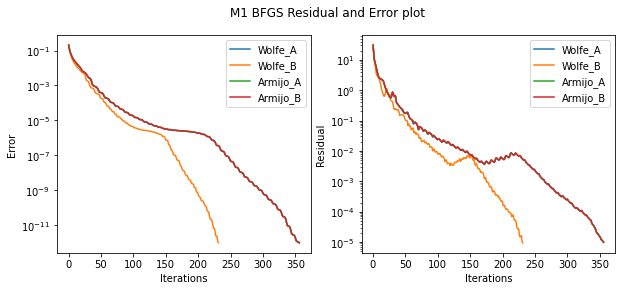
\includegraphics[scale=0.33]{bfgs/m1_o.png}\label{fig:bfgs_f1_o}}
  \hfill
  \subfloat[C-BFGS]{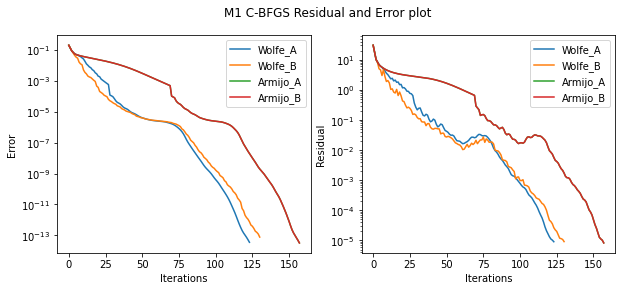
\includegraphics[scale=0.33]{bfgs/m1_c.png}\label{fig:bfgs_f1_c}}
  \caption{Relative error and residual plot for M1 matrix}
    \label{fig:err_bfgs_m1}
\end{figure}

In the case of the ill-conditioned matrix $\boldsymbol{M1}$, whose plots are displayed in Figure \ref{fig:err_bfgs_m1}, the cautious version of the BFGS algorithm seems to greatly outperform the original one in both the number of iterations need for convergence and the ultimate magnitude of the error. Again, the original BFGS appears to be \textit{mostly} invariant with respect to the type of line-search it employs, said invariance stands mostly evident for C-BFGS with respect to the employment of Armijo-type line search.
\\

\begin{figure}[H]
    \centering
    \subfloat[BFGS]{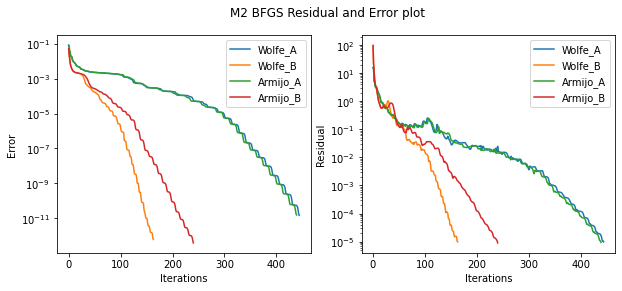
\includegraphics[scale=0.33]{bfgs/m2_o.png}\label{fig:bfgs_f2_o}}
  \hfill
  \subfloat[C-BFGS]{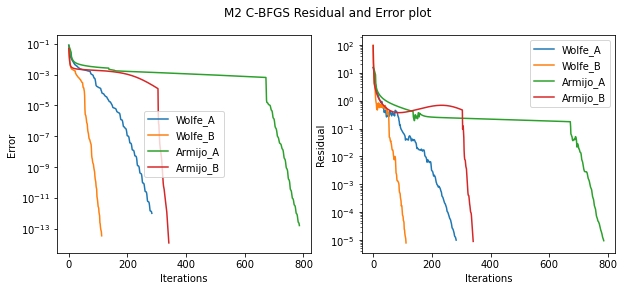
\includegraphics[scale=0.33]{bfgs/m2_c.png}\label{fig:bfgs_f2_c}}
  \caption{Relative error and residual plot for M2 matrix}
    \label{fig:err_bfgs_m2}
\end{figure}
Figure \ref{fig:err_bfgs_m2} displays the plots for the $\textbf{M2}$ matrix, While C-BFGS seems to outperform the original BFGS when emploing a Wolfe-type line search, the opposite of this phenomenon is observed when emploing an Armijo-type one. 
\\

\begin{figure}[H]
    \centering
    \subfloat[BFGS]{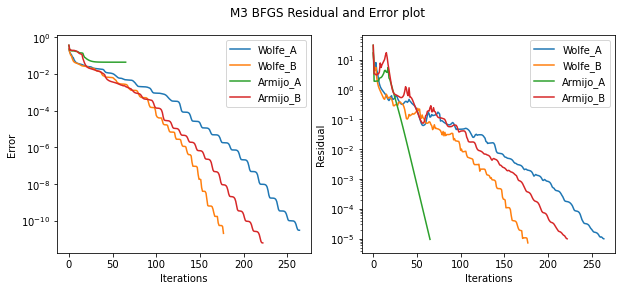
\includegraphics[scale=0.33]{bfgs/m3_o.png}\label{fig:bfgs_f3_o}}
  \hfill
  \subfloat[C-BFGS]{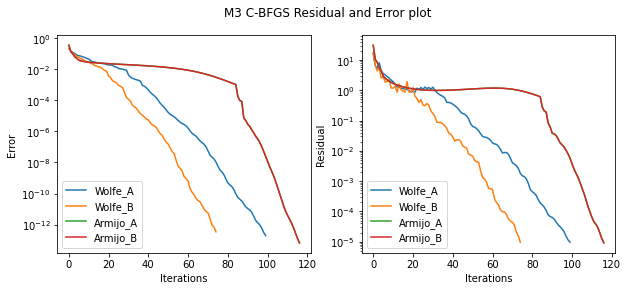
\includegraphics[scale=0.33]{bfgs/m3_c.png}\label{fig:bfgs_f3_c}}
  \caption{Relative error and residual plot for M3 matrix}
    \label{fig:err_bfgs_m3}
\end{figure}

\begin{figure}[H]
    \centering
    \subfloat[BFGS]{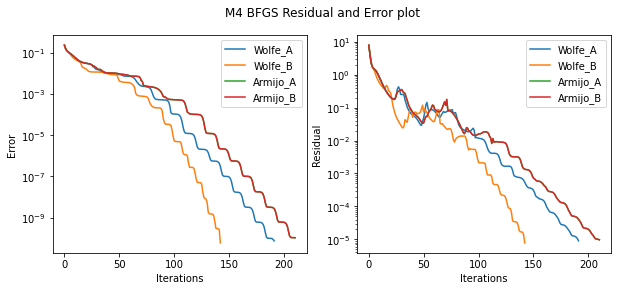
\includegraphics[scale=0.33]{bfgs/m4_o.png}\label{fig:bfgs_f4_o}}
  \hfill
  \subfloat[C-BFGS]{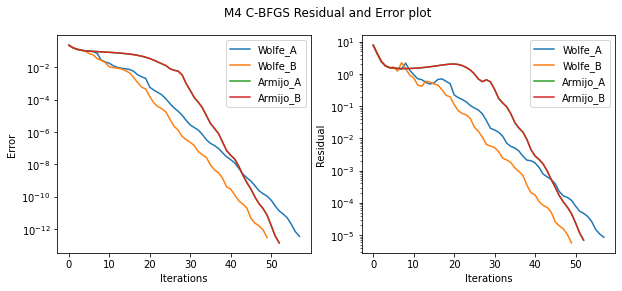
\includegraphics[scale=0.33]{bfgs/m4_c.png}\label{fig:bfgs_f4_c}}
  \caption{Relative error and residual plot for M4 matrix}
    \label{fig:err_bfgs_m4}
\end{figure}

\begin{figure}[H]
    \centering
    \subfloat[BFGS]{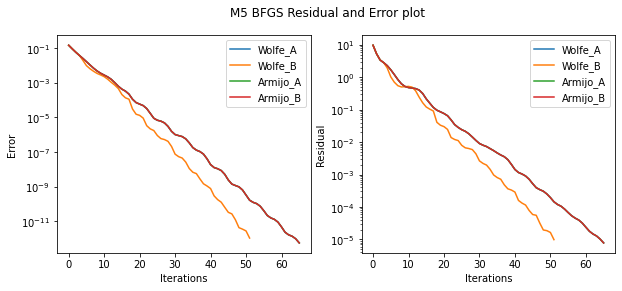
\includegraphics[scale=0.33]{bfgs/m5_o.png}\label{fig:bfgs_f5_o}}
  \hfill
  \subfloat[C-BFGS]{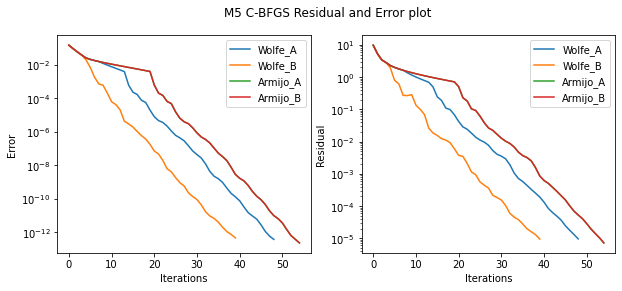
\includegraphics[scale=0.33]{bfgs/m5_c.png}\label{fig:bfgs_f5_c}}
  \caption{Relative error and residual plot for M5 matrix}
    \label{fig:err_bfgs_m5}
\end{figure}

 \ref{fig:err_bfgs_m3}, \ref{fig:err_bfgs_m4} and \ref{fig:err_bfgs_m5} confirm the better performance of C-BFGS regarding its application to the three randomly generated matrices. A relevant trend is also the one identifying Wolfe-type line search, especially the one employing the set of values for the $c_1$ and $c_2$ constants suggested by \cite{LiFukushimaA}, as the most efficient among its peers.\\ 
 
 One of the runs shown on Figure \ref{fig:bfgs_f3_o}, specifically the one using an Armijo-type line search with $c_1=0.0001$ in the search for $\textbf{M3}$'s norm, has shown to stop at a point of unusually high relative error. After performing additional tests with different starting points generated randomly and having actually verified their convergence to lower-error points, we established that the first outcome had to be dictated by an unlucky convergence at a local minimum. 

\subsubsection{Algorithms time and accuracy performance}
We now present the results of our comparison of the average running time and accuracy performance of both our BFGS and C-BFGS algorithms with respect to the Scipy's implementation of the former. Numpy's implementation of the matrix-norm function has been used to compute the error as the absolute difference between the value provided by said function and the solution provided by our algorithms, or the implementation from Scipy.
\\

The set of values utilized for the positive constants $c_1$ and $c_2$ are presented in the respective columns. Scipy's implementation of BFGS is based on an application of the Wolfe-type line search with default values for $c_1=1e-4$ and $c_2=0.9$.
\\

\begin{table}[H]
    \centering
    \begin{tabular}{||c c c c c c c||}
 \hline
 Matrix & Line-search & $c_1$ & $c_2$ & Average time & Relative Error & Iterations \\ [0.8ex] 
 \hline\hline
 M1 & Wolfe & 0.0001 & 0.9 & 50.2 s ± 276 ms & 1.01e-12 & 357 \\ 
 \hline
 M1 & Wolfe & 0.1 & 0.49 & 32.1 s ± 283 ms & 1.03e-12 & 232 \\ 
 \hline
 M1 & Armijo & 0.0001 & // & 47.8 s ± 250 ms & 9.87e-13 & 357 \\ 
 \hline
 M1 & Armijo & 0.1 & // & 47.6 s ± 1.5 s & 9.87e-13 & 357 \\ 
 \hline
 M2 & Wolfe & 0.0001 & 0.9 & 243 ms ± 11.3 ms & 1.46e-11 & 445 \\ 
 \hline
 M2 & Wolfe & 0.1 & 0.49 & 109 ms ± 18.3 ms & 6.11e-13 & 169 \\ 
 \hline
 M2 & Armijo & 0.0001 & // & 232 ms ± 19.1 ms & 1.55e-11 & 440 \\ 
 \hline
 M2 & Armijo & 0.1 & // & 128 ms ± 12.7 ms & 3.86e-13 & 241 \\ 
 \hline
 M3 & Wolfe & 0.0001 & 0.9 & 38.2 s ± 2.67 s & 3.08e-11 & 265 \\ 
 \hline
 M3 & Wolfe & 0.1 & 0.49 & 20.9 s ± 183 ms & 2.09e-11 & 172 \\ 
 \hline
 M3 & Armijo & 0.0001 & // & 7.75 s ± 113 ms & 0.04 & 66 \\ 
 \hline
 M3 & Armijo & 0.1 & // & 27.3 s ± 2.52 s & 6.32e-12 & 223 \\ 
 \hline
 M4 & Wolfe & 0.0001 & 0.9 & 112 ms ± 17.3 ms & 7.39e-11 & 192 \\ 
 \hline
 M4 & Wolfe & 0.1 & 0.49 & 91.6 ms ± 4.62 ms & 5.89e-11 & 143 \\ 
 \hline
 M4 & Armijo & 0.0001 & // & 109 ms ± 17 ms & 1.05e-10 & 211 \\ 
 \hline
 M4 & Armijo & 0.1 & // & 118 ms ± 17.5 ms & 1.05e-10 & 211 \\ 
 \hline
 M5 & Wolfe & 0.0001 & 0.9 & 37.4 ms ± 2 ms & 5.73e-13 & 66 \\ 
 \hline
 M5 & Wolfe & 0.1 & 0.49 & 34.3 ms ± 3.48 ms & 1.09e-12 & 52 \\ 
 \hline
 M5 & Armijo & 0.0001 & // & 34.1 ms ± 1.91 ms & 5.73e-13 & 66 \\ 
 \hline
 M5 & Armijo & 0.1 & // & 35.2 ms ± 3.07 ms & 5.73e-13 & 66 \\
 \hline
 \end{tabular}
    \caption{Time and accuracy performance for our implementation of the BFGS algorithm}
    \label{tab:performance_BFGS}
\end{table}

\begin{table}[H]
    \centering
    \begin{tabular}{||c c c c||}
 \hline
 Matrix & Average time & Relative Error & Iterations \\ [0.8ex] 
 \hline\hline
 M1 & 49.5 s ± 507 ms & 9.79e-13  & 422 \\ 
 \hline
 M2 & 46.7 ms ± 11 ms & 0.0002 &  78\\ 
 \hline
 M3 & 34.4 s ± 489 ms & 4.44e-11 & 294 \\ 
 \hline
 M4 & 33 ms ± 1.81 ms & 0.04 & 55 \\ 
 \hline
 M5 & 33.1 ms ± 1.86 ms & 7.26e-14 & 57 \\ 
 \hline
 \end{tabular}
    \caption{Time and accuracy performance for the Scipy's implementation of the BFGS algorithm}
    \label{tab:performance_off_shelf}
\end{table}

\begin{table}[H]
    \centering
    \begin{tabular}{||c c c c c c c||}
 \hline
 Matrix & Line-search & $c_1$ & $c_2$ & Average time & Relative Error & Iterations \\ [0.8ex] 
 \hline\hline
 M1 & Wolfe & 0.0001 & 0.9 & 12.1 s ± 148 ms & 3.53e-14 & 124 \\ 
 \hline
 M1 & Wolfe & 0.1 & 0.49 & 15.5 s ± 157 ms & 7.65e-14 & 131 \\ 
 \hline
 M1 & Armijo & 0.0001 & // & 12.9 s ± 140 ms & 3.21e-14 & 158 \\ 
 \hline
 M1 & Armijo & 0.1 & // & 12.7 s ± 147 ms & 3.21e-14 & 158 \\
 \hline
 M2 & Wolfe & 0.0001 & 0.9 & 149 ms ± 14.6 ms & 9.70e-13 & 284 \\ 
 \hline
 M2 & Wolfe & 0.1 & 0.49 & 64.2 ms ± 1.74 ms & 3.34e-14 & 113 \\ 
 \hline
 M2 & Armijo & 0.0001 & // & 198 ms ± 10.4 ms & 1.55e-13 & 787 \\ 
 \hline
 M2 & Armijo & 0.1 & // & 81.2 ms ± 2.29 ms & 1.15e-14 & 342 \\ 
 \hline
 M3 & Wolfe & 0.0001 & 0.9 & 9.32 s ± 205 ms & 1.94e-13 & 100 \\ 
 \hline
 M3 & Wolfe & 0.1 & 0.49 & 7.84 s ± 93.2 ms & 3.40e-13 & 75 \\ 
 \hline
 M3 & Armijo & 0.0001 & // & 4.83 s ± 60.9 ms & 6.59e-14 & 117 \\ 
 \hline
 M3 & Armijo & 0.1 & // & 4.76 s ± 75.6 ms & 6.59e-14 & 117 \\ 
 \hline
 M4 & Wolfe & 0.0001 & 0.9 & 32.7 ms ± 1.68 ms & 3.62e-13 & 58 \\ 
 \hline
 M4 & Wolfe & 0.1 & 0.49 & 31.3 ms ± 3.1 ms & 2.97e-13 & 50 \\ 
 \hline
 M4 & Armijo & 0.0001 & // & 21.5 ms ± 1.25 ms & 1.41e-13 & 53 \\ 
 \hline
 M4 & Armijo & 0.1 & // & 22.2 ms ± 1.79 ms & 1.41e-13 & 53 \\ 
 \hline
 M5 & Wolfe & 0.0001 & 0.9 & 33.7 ms ± 8.77 ms & 3.63e-13 & 49 \\ 
 \hline
 M5 & Wolfe & 0.1 & 0.49 & 30.3 ms ± 2.67 ms & 4.50e-13 & 40 \\ 
 \hline
 M5 & Armijo & 0.0001 & // & 35.2 ms ± 14.5 ms & 2.25e-13 & 55 \\ 
 \hline
 M5 & Armijo & 0.1 & // & 29.4 ms ± 1.66 ms & 2.25e-13 & 55 \\
 \hline
 \end{tabular}
    \caption{Time and accuracy performance for our implementation of the C-BFGS algorithm}
    \label{tab:performance_BFGS}
\end{table}











\section{Largest Eigenvalue Estimation via Arnoldi Iteration}
The following section describes our use of the Gram-Schmidt-style Arnoldi iteration to reduce a  matrix $\boldsymbol{A}^T\boldsymbol{A}$ to Hessenberg form and approximate its largest eigenvalue. The relationship between the norm of a matrix $\boldsymbol{A}$ and the spectral radius of its scalar product matrix $\boldsymbol{M}=\boldsymbol{A}^T\boldsymbol{A}$ is exploited in order to compute the former.\\

We start by introducing the Arnoldi Iteration algorithm with its proprieties.

\begin{algorithm}
\caption{Arnoldi Iteration}\label{alg:cap}
\begin{algorithmic}
\Procedure{Arnoldi}{$\boldsymbol{M} \in \mathbb R^{m \times n}, b \in \mathbb R^n,  k \in \mathbb N$}
\State $H = \text{matrix of zeros} \in \mathbb R^{m \times k+1}$
\State $q_1 = b/ \|b\|$
\For{$i=1,...,k$}
    \State $v=Mq_i$
    \For{$j=1,...,i$}
        \State $H_{ji}=q_j^*v$
        \State $v=v-H_{ji}q_j$
    \EndFor
    \State $H_{i+1,i}=\|v\|$
    \State $q_{i+1}= v/H_{i+1,i}$
\EndFor
\State \textbf{return} $H$
\EndProcedure
\end{algorithmic}
\end{algorithm}

The matrix $\boldsymbol{H}$ is an upper Hessenberg matrix  while the $\boldsymbol{Q}=[q_1,...,q_m]$ matrix contains the basis vectors of the Krylov subspace, both are incrementally constructed by the algorithm. The initial vector $\boldsymbol{b}$, soon normalized, is instead randomly built as is usual when applying the Arnoldi Iteration to the problem of estimating eigenvalues. 

At each new iteration, the algorithm construct a new basis vector $\boldsymbol{q}_{k+1}$, orthogonal to its predecessors, by using a modified Gram-Schmidt process.\\

By assuming $k < m$, we can consider $\boldsymbol{H}_k$, the upper Hessenberg matrix generated via $k$ iterations of the Arnoldi algorithm, as a low-rank approximation of matrix $\boldsymbol{M}=\boldsymbol{A}^T\boldsymbol{A}$. 

Its eigenvalues, usually called Ritz Values, are known to converge to the largest eigenvalues of $\boldsymbol{M}$, as we will soon prove.\\
By using the Arnoldi Iteration for the construction of increasingly more complex approximations of $\boldsymbol{A}^T\boldsymbol{A}$, we can identify an exact, if not nearly so, value for the largest eigenvalue of said matrix and therefore compute the norm of the original matrix $\boldsymbol{A}$ according to the spectral radius property analyzed in (2.1).\\
What follows is our propose for the algorithm performing the aforementioned norm estimation. 
\begin{algorithm}
\caption{Norm Estimation based on the Arnoldi Iteration}\label{alg:cap}
\begin{algorithmic}
\Procedure{Arnoldi-Norm}{$\boldsymbol{M} \in \mathbb R^{m \times n}$}
\State $b = \text{arbitrary vector}$
\State $k=1$
\State $H_1 = \textbf{ARNOLDI}(M,b,1)$
\State $\theta_1 = \max{(\text{eig}(H_1)})$
\Repeat
    \State $k = k +1$
    \State $H_k = \textbf{ARNOLDI}(M,b,k)$
    \State $\lambda_k = \max{(\text{eig}(H_k)})$ \Comment{Largest Ritz-Value Estimation}
\Until{$\|\lambda_k - \lambda_{k-1} \| < \epsilon$} \Comment{Check for Convergence}
\State \textbf{return} $\sqrt{\lambda_k}$\Comment{The norm of $A$ is computed from $\lambda_k$ according to (2.1)}
\EndProcedure
\end{algorithmic}
\end{algorithm}

\subsection{Convergence of the Algorithm} 
The following section describes the Convergence of the Arnoldi method for our Eigenvalue Estimation .
We saw the Convergence of the Arnoldi method in two cases.
In the first case If there is a lucky breaks down at step $\boldsymbol{n}$.
Recall that given a Matrix $\boldsymbol{M}$ the Arnoldi method produce 
\begin{equation}
     MQ_n = Q_{n+1}H_n 
\end{equation}
we can rewrite equation 5.1 as  
    \begin{equation}
     MQ_n = Q_nH_n +q_{n+1}\beta_{n+1,n} \epsilon_n^T   
\end{equation} ${H_n}$ is without the last row and ${\epsilon_n^T }$ is a vector with all element  0 expect the last entity at n is 1. \\
We said luck break down happen when ${\beta_{n+1,n}}$ = 0 and then equation 5.2 reduce to  
\begin{equation}
     MQ_n = Q_nH_n 
\end{equation} in such a case when luck break down happen the eigenvalue value of ${H_n}$ is a subset of the eigenvalue ${M}$.\\ proof as follows:\\
For every  eigenvalue eigenvector pair  ${H_n V}$ = ${\lambda V}$ , ${M x}$ = ${\lambda x}$, ${x}$ = ${Q_n V}$ i.e (${\lambda}$,${x}$) eigenvalue eigenvector pair M. \\
\begin{equation}
     MQ_n = Q_nH_n 
\end{equation}
\begin{equation}
     MQ_nV = Q_nH_nV = Q_n\lambda V  
\end{equation}
\begin{equation}
     MQ_nV = \lambda Q_n V 
\end{equation} 
where ($Q_n$V, $\lambda$) are  eigen pair of M which implies  the eigenvalue of $\boldsymbol{H}$ is subset of the eigenvalue of M.\\
 
The second case is when there is no lucky break down  at $\boldsymbol{n}$ steps, eigenvalue and eigenvector of ${H}$ is a good approximation of our matrix ${M}$ and we can check this by computing the difference of eigenvector and eigenvalue of M and taking the norm should equal to 0 as such  $\|Mx-\lambda x\|$ = 0.  




\subsection{Complexity of the Arnoldi Iteration}

We now compute the complexity of running $k$ steps of the Arnoldi Iteration when applied to a matrix $\boldsymbol{P} \in \mathbb R^{m \times n}$ and a vector $\boldsymbol{b} \in \mathbb R^m$. 

The Arnoldi Iteration entails $k$ products with the $\boldsymbol{M}$ matrix. The cost of these products, assuming the sparsity of matrix $\boldsymbol{M}$, is $O(k \cdot nnz(\boldsymbol{M}))$, where $nnz(\boldsymbol{M})$ represents the total number of non-zero elements in $\boldsymbol M$. \\

The scalar product $h_{ji}=q_j^*v$ and linear combination of vectors $v=v-h_{ji}q_j$ are instead performed $O(k^2)$ times for a total cost of $O(m \cdot k^2)$.\\  

Additionally, the vector-norm operation $h_{i+1,i}=\|v\|$ and the vector scalar division $q_{i+1}= v/h_{i+1,i}$ are performed $k$ times for a total cost of $O(2\cdot k \cdot 2m) \approx O(k\cdot m)$ operations.  \\

Finally, the total cost of performing $k$ steps of the Arnoldi Iteration, in the case of a sparse $\boldsymbol{A}^T \boldsymbol{A}$ matrix, is:
\begin{equation}
    C(ARNOLDI)= O(k \cdot m \cdot nnz(\boldsymbol{M})) + (m \cdot k^2) + O(k\cdot m)= O(m\cdot k^2)
\end{equation}  \\

\subsection{Performance of Algorithm}
In this section we provide an analysis of the performance of Arnoldi algorithms  when applied to the experimental setup described in Section 3.4. In addition we perform $\boldsymbol{A}^T\boldsymbol{A}$ on {\textbf{M3}} ,{\textbf{M4}} and $\boldsymbol{AA}^T$ on {M2},{M5} to make them symmetric.
\subsubsection{Algorithm time performance}
We evaluated the running time performance of our algorithm and compared the accuracy of the result with numpy linear algebra implementation of a method norm \footnote{https://numpy.org/doc/stable/reference/generated/numpy.linalg.norm.html}. The following table summarises the running time of our implementation compared to the numpy tool. The error column represents the absolute difference between the solution provided by our algorithm and the numpy norm library.
\begin{table}[hbt!]
    \centering
    \begin{tabular}{||c c c c c||}
 \hline
 Matrix & Arnoldi & np.linalg.norm & Error & Iterations \\ [0.8ex] 
 \hline\hline
 M1 & 23.9 s ± 4.26 s  & 592 ms ± 18.5 ms & 2.86e-11  & 58 \\ 
 \hline
 M2 & 1.84 s ± 384 ms  & 201 ms ± 273 ms & 0.21 & 14\\
 \hline
 M3 & 5.83 s ± 208 ms & 11.8 ms ± 1.78 ms & 1.52e-12 & 35 \\
 \hline
  M4 & 636 ms ± 62.9 ms & 1.5 ms ± 241 µs & 3.6e-11 & 22 \\
 \hline
 M5 & 952 ms ± 152 ms & 6.2 ms ± 198 µs & 3.52e-11 & 19 \\
 \hline
\end{tabular}
    \caption{ Arnoldi Time performance}
    \label{tab:my_label}
\end{table}

From table 7, we can observe that the error, which is difference between the algorithm result and off the shelf solver solution,  indicates that the result provided by the algorithm is very close to the result provided by the off the shelf solver except for \textbf{M2} . We can observe that the algorithm failed to reach convergence on $\boldsymbol M2$ due to not enough number of  iterations. We analyzed by increasing the number of iterations and after taking too much time, the algorithm failed to converge. This could be due to the matrix eigenvalues being not well separated.

\subsubsection{Algorithm convergence rates}
We examined the convergent rate of the algorithm by comparing the Ritz values  to the exact eigenvalues.  We took the first 5 Ritz values of our algorithm and compared them to the corresponding exact eigenvalues calculated  with numpy linear algebra implementation of a method eig \footnote{https://numpy.org/doc/stable/reference/generated/numpy.linalg.eig.html}.
The following plots Figure 11 show  the convergent rate (as the absolute error  $|\lambda^{(n)} - x|$ ) as a function of the number of iterations \cite[pg.~261-265]{qr}. The algorithm converges fast for  all matrices and  we observe that the biggest  eigenvalue  is converging the fastest. 
\begin{figure}[H]
    \centering
    \subfloat[M1]{{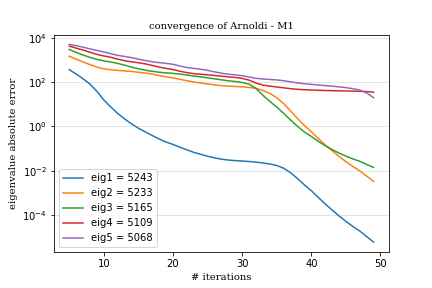
\includegraphics[width=6cm]{cgd/M1_a.png} }}
    \qquad
    \subfloat[M2]{{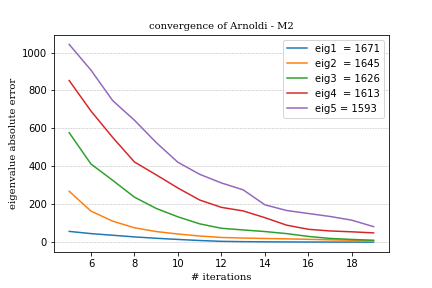
\includegraphics[width=6cm]{cgd/M2_a.png} }}
    
    \label{fig:example}
    \qquad
    \subfloat[M3]{{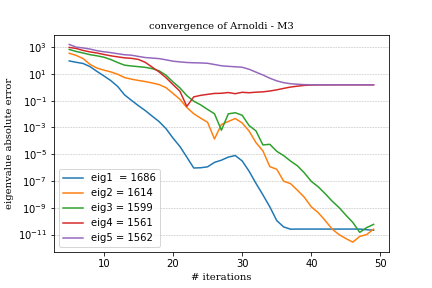
\includegraphics[width=6cm]{cgd/M3_a.png} }}
    \centering
    \subfloat[M4]{{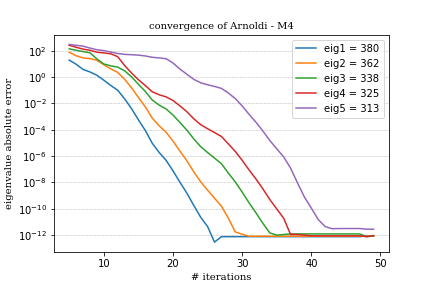
\includegraphics[width=6cm]{cgd/M4_a.png} }}
    \qquad
    \subfloat[M5]{{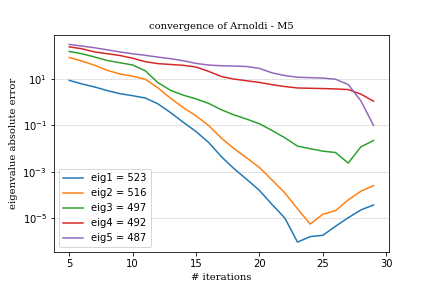
\includegraphics[width=6cm]{cgd/M5_a.png} }}
   
    \caption{ Arnoldi convergence rates}
    \label{fig:example}
    
    \label{fig:example}

    
\end{figure}

\section{ Arnoldi future improvement }
We observed that Arnold algorithm is the slowest compared to BFGS and CGD. Theoretically the method suffers from slow convergence when the eigenvalues are not well separated. The following section provides suggestions on how to accelerate the convergence of the method. The first method is based on restarting, it is a way of repeating a k-step arnoldi iteration after improving the starting vector ${v_0}$ . A rapid convergence should occurs if we choose the starting vector ${v_0}$ of the arnoldi process carefully.\\

\textbf{Lemma 6.1 (Lemma 2.1 in \cite{caho}):} if $v_0$ \in $\big\{\boldsymbol{W}_k \big\} $,where  $\boldsymbol{S}_k $  \in   $\mathbb{C}^{m \times n}$ and $\boldsymbol{A}\boldsymbol{W}_k = \boldsymbol{W}_k\boldsymbol{G}_k$ for some $\boldsymbol{G}_k$ \in   $\mathbb{C}^{k \times k}$  then 
\begin{equation}
  \mathcal{K}\big(\boldsymbol{A},\boldsymbol{v}_0;\boldsymbol{k}\big) \supset Span \big\{\boldsymbol{W}_k \big\} 
\end{equation}
and an arnoldi process with ${v}_0$ as the staring vector terminate in k or fewer steps. \\ 

Avoiding building a large Krylov subspace is another way to improve the speed of convergence, this again implies to initially carry out only k steps of Arnoldi iteration. If the k-dimension Krylov subspace fails to provide an accurate approximations, as it happened in the case of $\boldsymbol{M2}$, then recomputing an k-step Arnoldi factorization using a modified starting vector actually improves the convergence. This version of Arnoldi based on modifying the starting vector and refactorization procedure is called Restarted Arnoldi.\\

A strategy to implementing the new starting vector $v_0$ is to replace $v_0$ with $\Psi$(A)$v_0$ where $\Psi$(A) is a function constructed to filter out the unwanted eigencomponents from $v_0$. 
\begin{equation}
    v_0 \leftarrow \Psi(A)v_0 
\end{equation}
Restarted Arnoldi requires us to explicitly compute $v_0$ but the Implicitly Restarted Arnoldi algorithm  (IRA) avoids to compute $\Psi$(A)$v_0$ directly and the new starting vector emerges as a by-product of a sequence of implicit QR updates.  \\

Another method we can consider is a spectral transformation which is based on the idea of transforming the original eigenvalue problem, with a polynomial or rational transformation, into one that is easier to solve.
\section{Conclusion}
We now provide an overall comparison among the three methods and their variants.\\

In terms of speed the Conjugate Gradient method has showed the best performance, with the Fletcher-Reeves variant slightly outperforming the Rolak-Ribière one. The original version of the BFGS algorithm instead, while still being the slowest method for application concerning ill-conditioned matrices, like \textbf{M1}, has shown better speed than Arnoldi's take on the problem. Lastly, C-BFGS, the more cautious version of the algorithm, has showed to outperform its inspiration in all scenarios. 
\\

In order to provide a comparison of the results of the application of the methods on ill-conditioned matrices, we may need to account for the application-specific trade-off between accuracy and speed. C-BFGS has shown to be the most accurate but the CGD method has proved to be the fastest, on ill-conditioned matrix as on the other ones, while still providing a relatively good accuracy.

\newpage
\medskip

\printbibliography

\end{document}
